%%%%%%%%%%%%%%%%%%%%%%%%%%%%%%%%%%%%%%%%%%%
%%% DOCUMENT PREAMBLE %%%
%This template was adapted from a template by Roza Aceska.
\documentclass[12pt]{report}
\usepackage[english]{babel}
%\usepackage{natbib}
\usepackage{url}
\usepackage[utf8x]{inputenc}
\usepackage{amsmath}
\usepackage{graphicx}
\usepackage{parskip}
\usepackage{fancyhdr}
\usepackage{vmargin}
\usepackage{caption}
\usepackage{subcaption}

\usepackage{tabularx}
\usepackage{xcolor,colortbl}
\newcommand{\notimportant}{\cellcolor{black!10}x} 
\usepackage{hyperref}
\usepackage{cleveref}
\usepackage{float}

\setmarginsrb{3 cm}{2.5 cm}{3 cm}{2.5 cm}{1 cm}{1.5 cm}{1 cm}{1.5 cm}

\title{Report Assignment Part 2}
% Title
\author{}						
% Author
\date{17.07.2020}
% Date

\makeatletter
\let\thetitle\@title
\let\theauthor\@author
\let\thedate\@date
\makeatother

\pagestyle{fancy}
\fancyhf{}
\rhead{\theauthor}
\lhead{\thetitle}
\cfoot{\thepage}
%%%%%%%%%%%%%%%%%%%%%%%%%%%%%%%%%%%%%%%%%%%%
\begin{document}

%%%%%%%%%%%%%%%%%%%%%%%%%%%%%%%%%%%%%%%%%%%%%%%%%%%%%%%%%%%%%%%%%%%%%%%%%%%%%%%%%%%%%%%%%

\begin{titlepage}
	\centering
    \vspace*{0.5 cm}
  \begin{center}    \textsc{\Large   Adavanced Process Mining SS20}\\[2.0 cm]	\end{center}
	\rule{\linewidth}{0.2 mm} \\[0.4 cm]
	{ \huge \bfseries \thetitle}\\
	\rule{\linewidth}{0.2 mm} \\[1.5 cm]
	
  \begin{minipage}{0.48\textwidth}
    \begin{flushleft} \large
      \emph{Submitted To:}\\
      Tobias Brockhoff\\
      Lisa Mannel\\
      Sebastiaan J. van Zelst MSc PhD\\
    \end{flushleft}
  \end{minipage}~
  \begin{minipage}{0.48\textwidth}
    \begin{flushright} \large
			\emph{Submitted By:} \\
      Sezin Maden (354463) \\
      Bruno Machado Pacheco (403532)  \\
      Tom-Hendrik Hülsmann (355773)
		\end{flushright}
	\end{minipage}\\[2 cm]
	
\end{titlepage}

%%%%%%%%%%%%%%%%%%%%%%%%%%%%%%%%%%%%%%%%%%%%%%%%%%%%%%%%%%%%%%%%%%%%%%%%%%%%%%%%%%%%%%%%%

\renewcommand{\thesection}{\arabic{section}}

\section{Q1. Preliminary Analysis}

\paragraph{\textbf{a)}}
We begin our analysis by creating two sub-logs of the original event log. One sub-log that contains all cases that did have an appeal and one sub-log containing all cases that did not have an appeal. The distinction between such cases is made based on events that are related to appeals. We know that there are two ways in which an offender can appeal. There either is an appeal to the prefecture or to a judge. The two relevant events that indicate an appeal on the side of the police department are \texttt{Appeal to Judge} and \texttt{Send Appeal to Prefecture}. The two sub-logs are created by filtering the original log based on these events using pm4py. Traces that contain either of these events are either discarded or kept depending on the sub-log.

\paragraph{\textbf{b)}}
For the three logs obtained in the previous step, we compute some core descriptive metrics. All of the resulting values can be found in \ref{tab:1b}.
\begin{table}[H]
\centering
\begin{tabular}{|l|l|l|l|l|}
	\hline \textbf{Metric} & \textbf{Complete} & \textbf{Only Appeals} & \textbf{Without Appeals} \\
	\hline Number of Traces & 150,370 & 4,513 & 145,857\\
	\hline Number of Variants & 231 & 170 &61\\
	\hline Number of Events & 561,470 & 29,724 & 531,746\\
	\hline Average Trace Length & 3.73 & 6.59 & 3.65\\
	\hline First Event Date & 01.01.2000 & 03.01.2000 & 01.01.2000\\
	\hline Last Event Date & 18.06.2013 & 14.06.2013 & 18.06.2013\\
	\hline Number of Activities & 11 & 11 & 9 \\
	\hline Traces with Duplicate Activities  & 0.0812 \% & 0.0252 \% & 0.0843 \%\\
	\hline
\end{tabular}
\caption{Some basic Metrics of the three event logs.}
\label{tab:1b}
\end{table}
The \emph{Number of Traces}, \emph{Number of Events} and \emph{Number of Activities} metrics were obtained through the \emph{Log Summary} feature of ProM. The \emph{Number of Variants}, \emph{Average Trace Length} and \emph{First/Last Event Date} were computed using the \emph{Explore Event Log} feature of ProM. Additionally the number of traces that are containing duplicate activities were computed using a custom Python script.

\paragraph{\textbf{c)}}

An overview of the relative frequency of all activities in the three logs can be seen in figure \ref{fig:activity_frequencies}. The raw frequency values can be found in the appendix in table \ref{tab:1c_absolut} and table \ref{tab:1c_relative}. The values were obtained using the \emph{Log Summary} feature of ProM. 
\begin{figure}[H]
  \centering
  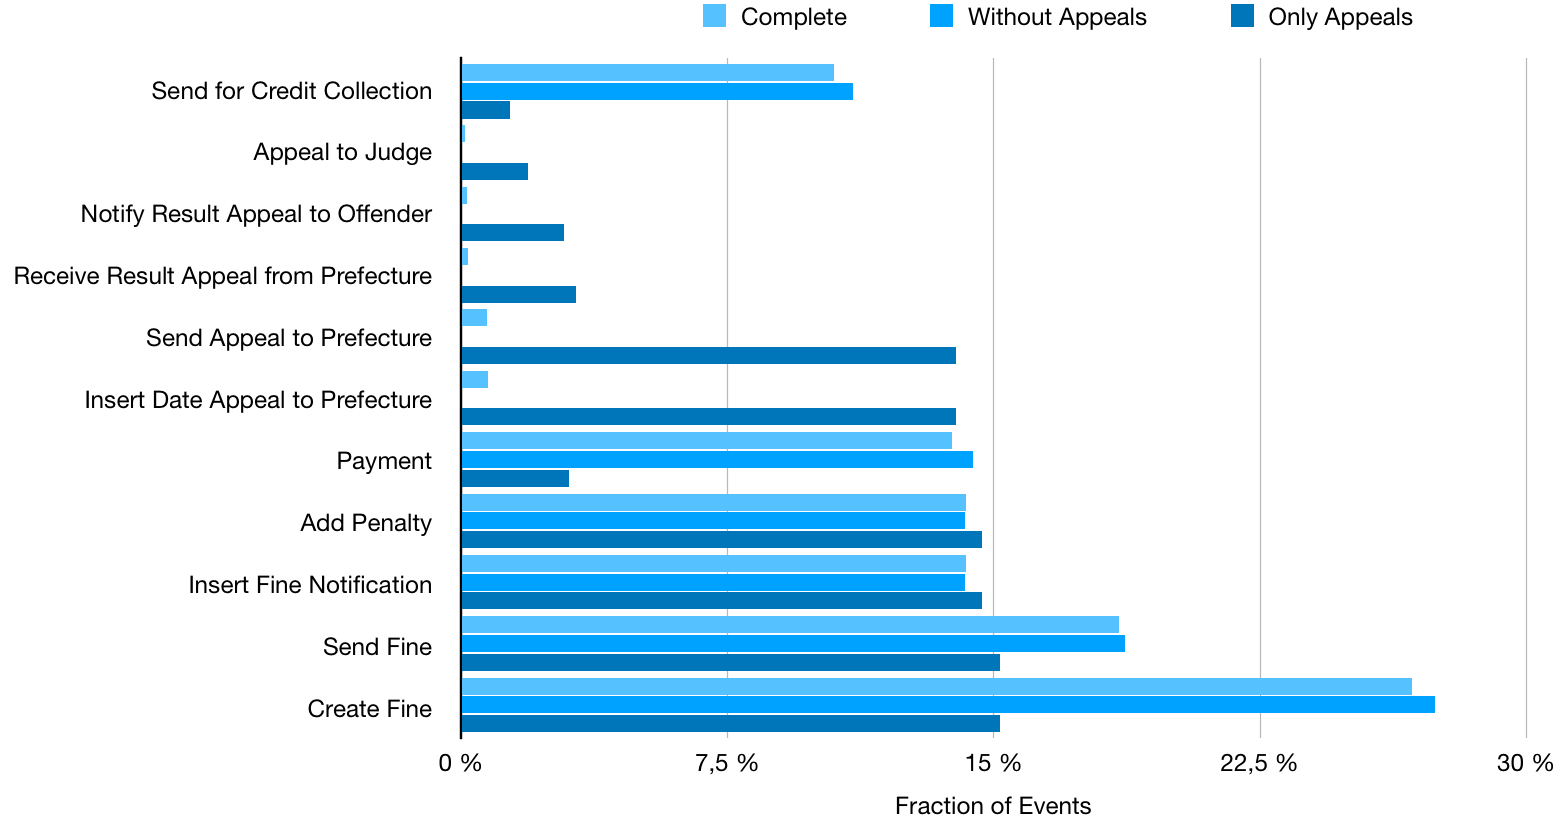
\includegraphics[width=\textwidth]{figures/activity_frequencies.png}
  \caption{The fraction of events of each log grouped by activity.}
  \label{fig:activity_frequencies}
\end{figure}

Also using the ProM \emph{Log Summary} feature, it was found that for all three event logs, 100\% of the traces start with the \texttt{Create Fine} activity. The relative frequencies of end activities can be found in figure \ref{fig:end_frequencies}. The exact values for the end activity frequencies can be found in the appendix in table \ref{tab:1c_end}. 
\begin{figure}[H]
  \centering
  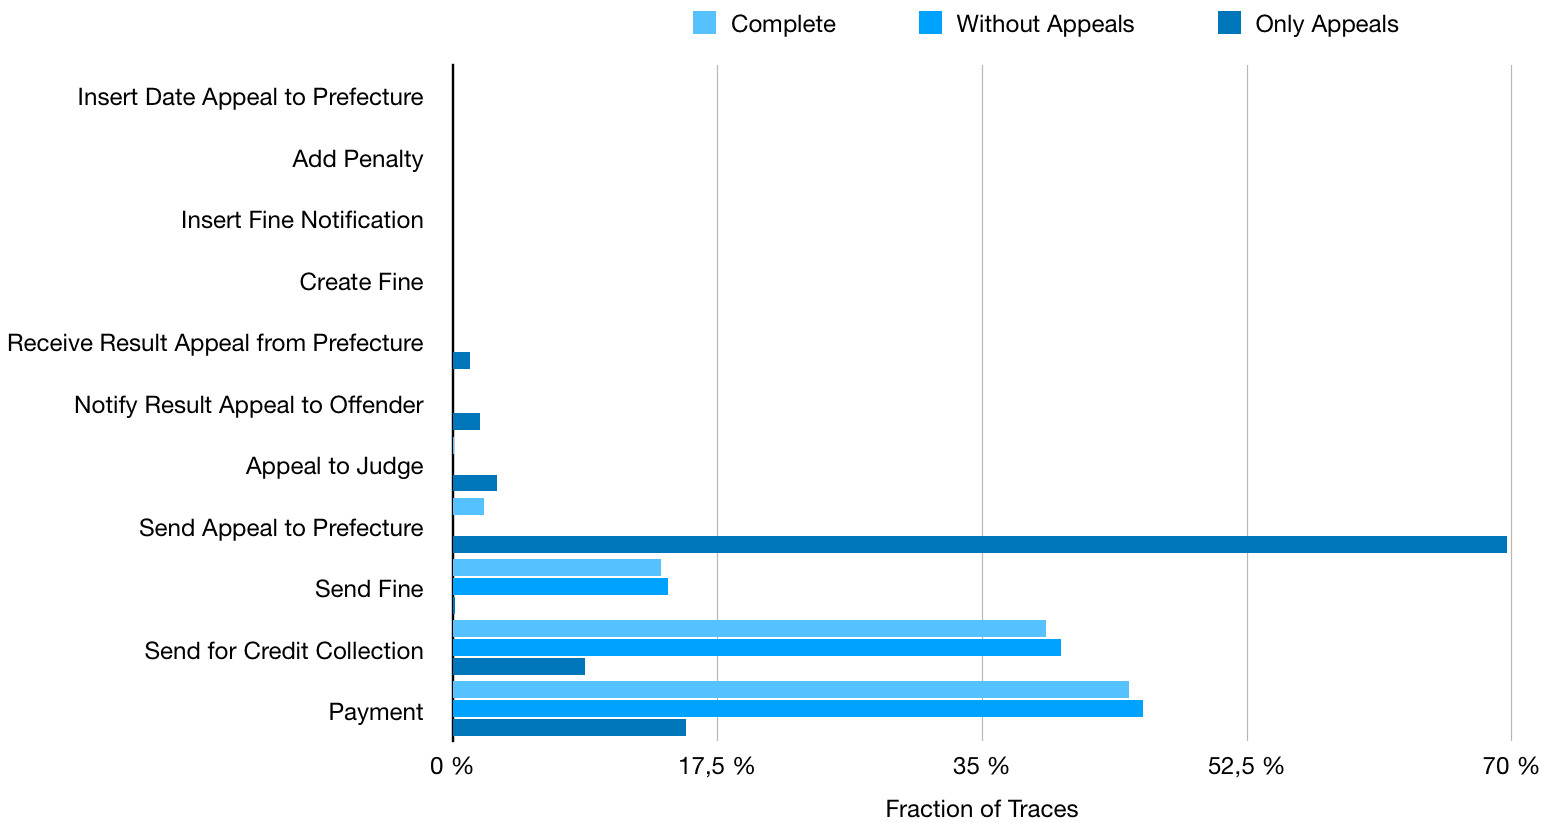
\includegraphics[width=\textwidth]{figures/end_frequencies.png}
  \caption{The fraction of Traces that end with the specified activity in each of the three event logs.}
  \label{fig:end_frequencies}
\end{figure}

\paragraph{\textbf{d)}} In order to to be able to see the different activity types over time, two dotted charts over the events were created. This was done by importing the filtered event log, containing only cases that did not have an appeal, into ProM. There, the \emph{LogProjection} plugin was used in order to create the two visualizations. The first chart that can be seen in figure \ref{fig:dotted_timestamp} shows the different activity types on the y-axis.
For each event, a dot is visible at the point in time when the event occurred. We can therefore observe which types of activities were performed at which time over the whole timespan of the log. In general we can see that there are two main types of activities. Those activities that are performed constantly throughout the year, and those that only occur infrequently. The continually performed activities consist of \texttt{Add Penalty}, \texttt{Create Fine}, \texttt{Insert Fine Notification}, \texttt{Payment} and \texttt{Send Fine} activities. Of those, the \texttt{Create Fine} and \texttt{Payment} activities have no gaps and are therefore always performed. The remaining continuous activities show some gaps over the years. These gaps do not seem to follow a particular pattern and are spread throughout the year. However we see, that the gaps of these activities coincide with each other somehow. The \texttt{Insert Date Appeal to Prefecture}, \texttt{Notify Result Appeal to Offender}, \texttt{Receive Result Appeal from Prefecture} and \texttt{Send for Credit Collection} activities occur much less frequent. The \texttt{Send for Credit Collection} activity seems to only occur once every year, mostly near the beginning or end of the year. The \texttt{Notify Result Appeal to Offender} and \texttt{Receive Result Appeal from Prefecture} activities only start appearing for the first time in 2007, in contrast to the other activities which occur from the beginning of the log. This suggest that they represent a new branch of the process that was introduced in 2007.
\begin{figure}[H]
  \centering
  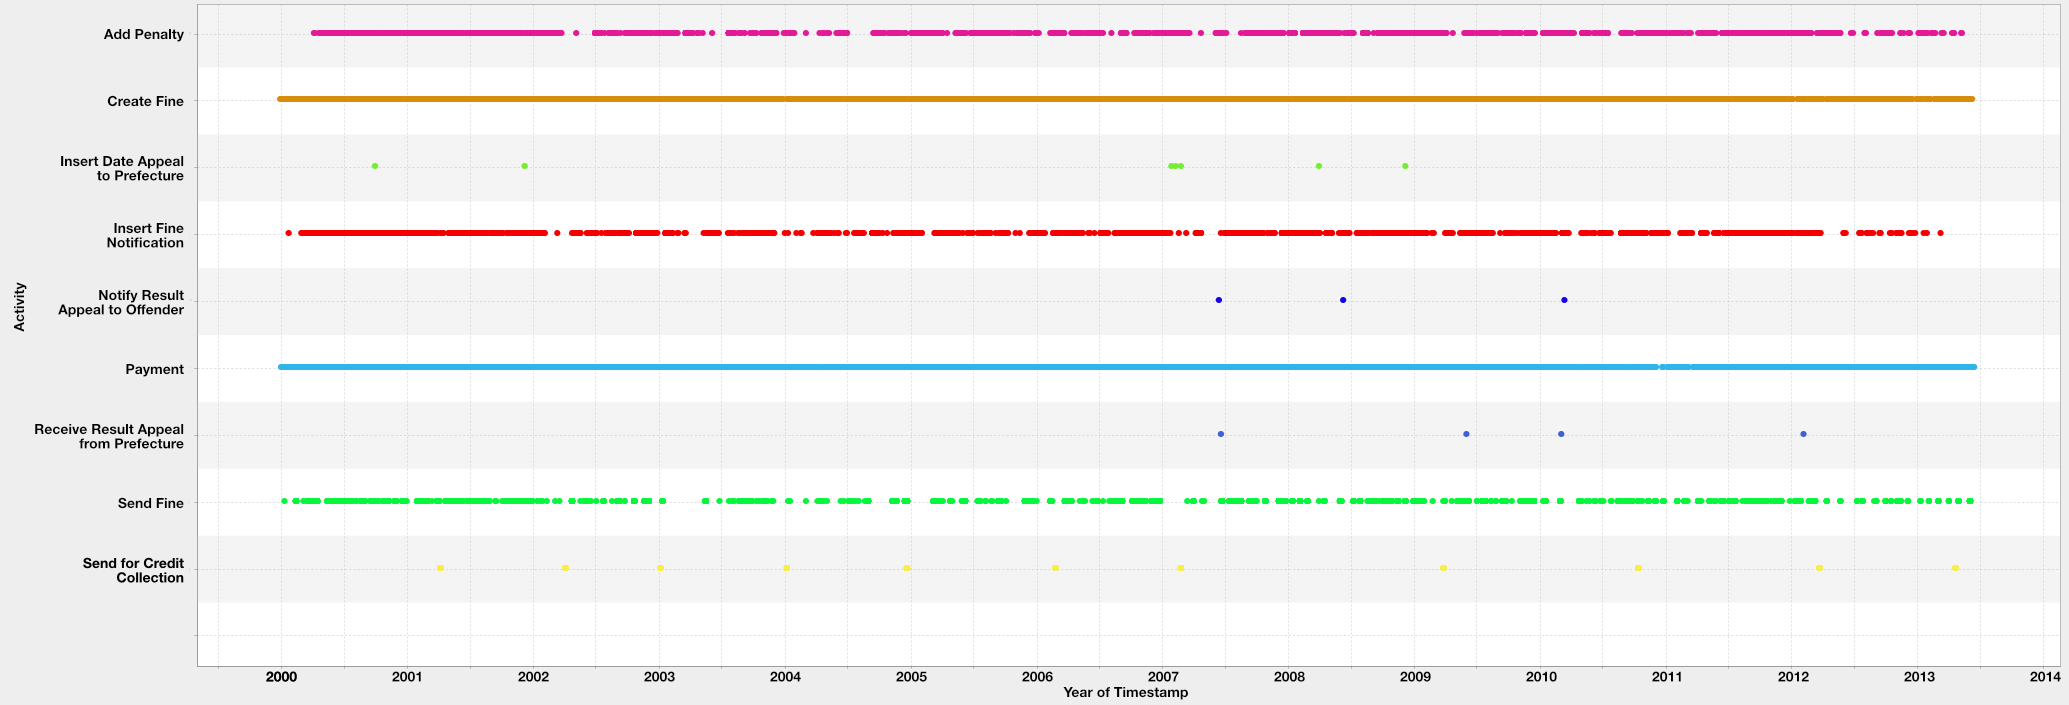
\includegraphics[width=\textwidth]{figures/dotted_timestamp.png}
  \caption{Event occurrences for cases without an appeal, grouped by activity type over time.}
  \label{fig:dotted_timestamp}
\end{figure}

The second chart that can be seen in figure \ref{fig:dotted_duration} also shows the different activity types on the y-axis. However the events are now plotted over the case duration at the time that the event occurred. This case duration metric was automatically computed by the used \emph{LogProjection} plugin. We see that \texttt{Create Fine} is always the first event of every case, as was already discovered in \textbf{c)}. The activity is therefore only observable at the beginning of the chart. \texttt{Send for Credit Collection} activity only starts after almost a full year of case duration and is the activity that is performed the latest in most cases. The first activity after one year can be explained with the findings from the previous chart, where it was discovered that the activity is only performed once a year. The \texttt{Payment} activity also has some events performed in late stages of the process instances, but is also frequent throughout all case durations. The other activities are mostly performed within the first year of an active case. The \texttt{Notify result Appeal to Offender} activity is always performed before the \texttt{Receive Result Appeal from Prefecture} activity. Overall we can see that the activities that are performed directly by the police department occur earlier in the cases or in cases that have an overall shorter duration. Activities that are depending on the offender and are related to payments appear at the very end of the case. The longest case durations are therefore caused by cases in which the offender makes a delayed payment. It is also visible that the frequent events are mostly spread across the whole range of case durations, with only a small reduction towards the extremely long case durations. This suggests that there are no peaks in case duration and there is an almost equal distribution of case durations over the timeframe.

\begin{figure}[H]
  \centering
  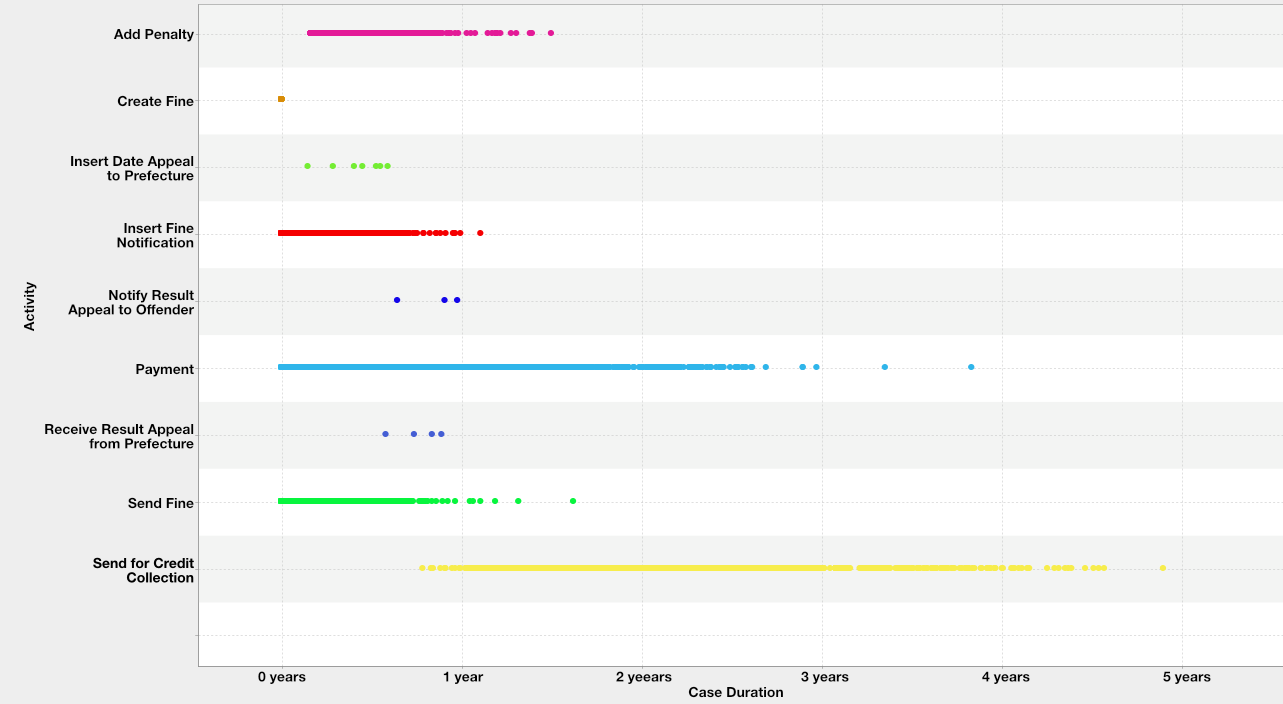
\includegraphics[width=\textwidth]{figures/dotted_duration.png}
  \caption{Event occurrences for cases without an appeal, grouped by activity type over the case duration at the time the event occurred.}
  \label{fig:dotted_duration}
\end{figure}

\paragraph{\textbf{e)}}

Based on table \ref{tab:1b} we can now compare the three logs according to some basic metrics. We see that the majority of
cases do not contain any appeal, with only around $3\%$ of the traces having an appeal. The average trace length of appeal cases is almost twice as long as for cases without appeal. Because of this, the cases are over represented regarding the number of events, with about $5\%$ of events in the original log being related to appeal cases. Using figure \ref{fig:activity_frequencies} we observe that most of these appeal cases are appeals to the prefecture. There are seven times as many appeals to the prefecture as there are appeals to a judge.  The variety of traces is much higher in the log containing only appeals. On average there are 100 times more traces for each variant in the log without appeals compared to the log with appeals. This means that a majority of trace variety in the log is explained by only a small number of traces with an appeal. This can be explained by the longer average trace length of these cases, which leads to more variant possibilities. Although the log with only appeals has a higher average trace length, it contains far less traces with duplicate activities than the other two logs, which is surprising. This can probably be explained by the fact that appeals processes involve additional events that are not possible for non appeals processes. We see that the original log has the same timeframe as the log without appeals. The log consisting of only appeals cases however starts two days later and ends four days prior. This can most likely be explained by the lower amount of cases that have an appeal, so that in the missing time, no events for such cases occurred. The number of activities is the same for the original log and the log containing only appeals cases. This means that there are no activities that are only performed for cases without appeals. As expected there are less activities in the log containing no appeals, as the events on which the filtering was based are no longer present.

In addition to the above findings, a closer look was given at the relative frequencies of specific activities in figure \ref{fig:activity_frequencies} and figure \ref{fig:end_frequencies}. As mentioned above we observe that the \texttt{Appeal to Judge} and \texttt{Send Appeal to Prefecture} activities are missing from the log without appeals because of the filtering. However there are still some activities left that are related to the appeals process and in theory should therefore only present in the log containing the appeals. These activities are \texttt{Insert Date Appeal to Prefecture}, \texttt{Receive Result Appeal from Prefecture} and \texttt{Notify Result Appeal to Offender}. A closer inspection of these traces reveals that in half of the instances, a payment was made directly after the \texttt{Insert Date Appeal to Prefecture} activity. This suggests that the offender was planning on appealing, but payed the fine before the appeal was sent to the prefecture. These traces are therefore most probably correct and are correctly assigned to the sub-log as indeed there was no appeal.  However in the other half of cases, the appeals process was complete, with receiving a result from the prefecture and notifying the offender. In these cases only the \texttt{Send Appeal to Prefecture} activity is missing, which suggests that these are recording errors in the log, because it is not possible to receive an answer from the prefecture without sending the appeal first. So most probably it was missed to record the sending activity.

An open question that could point to a possible problem is the high amount of traces containing \texttt{Send for Credit Collection} in the log without appeals. Especially when keeping in mind that this activity is batched together. It is very likely that the average case duration could be reduced if there were less cases where the fine has to be collected externally. The same observation can also be made in figure \ref{fig:end_frequencies}. Furthermore, in the cases without appeals there are many traces ending with a \texttt{Send Fine} activity, which points to a high number of unpaid fines. Further analysis should investigate if this suspicion is true and what can be done to counter it. Regarding the end activities it is also interesting that of the appeal cases, almost $70\%$ end with the \texttt{Send Appeal to Prefecture} activity. This is unexpected, as this is not a wanted end activity. This leads to the assumption that these cases are not yet finished and are still waiting for the next event to occur. To check this, we look at the distribution of these traces over time. If these are cases that were not yet finished before the end of the considered timeframe, we would expect them to pool at the end of the timeframe. This is however not the case, the cases are spread evenly over the timeframe. Therefore the cases are most probably actually finished. Further investigation reveals that in most cases where the end activity was not \texttt{Send Appeal to Prefecture}, an actual payment was made or the case was sent for credit collection. This suggests that the case is only passed back to the police department in cases in which the appeal is discarded. This means that the appeals of the cases ending in \texttt{Send Appeal to Prefecture} were most probably successful appeals.

\section{Q2. Discovery and Conformance}

\paragraph{\textbf{a)}}
As discovered in Q1 there are remaining appeal related activities in the filtered version of the event log that should not contain any appeals. We identified two types of traces that contain such events. One type where we assume that the \texttt{Send Appeal to Prefecture} activity was falsely not recorded and one type where the offender decided to pay the fine before the appeal was sent. The former traces are not correctly assigned to the log without appeals. In order to obtain a meaningful process model for cases without appeals they are therefore removed from the log before mining for a process model. The other type of traces are kept, in order to represent initiated appeals that were not actually sent.

In order to obtain a process model for the process without appeals, the Inductive Miner was applied. It was chosen because it can discover more complex process constructs than for example the Alpha Miner and can also represent infrequent behaviour (such as the \texttt{Insert Date Appeal to Prefecture}) activity discussed above. The discovered model can be found in figure \ref{fig:im_no_appeals}.
\begin{figure}[H]
  \centering
  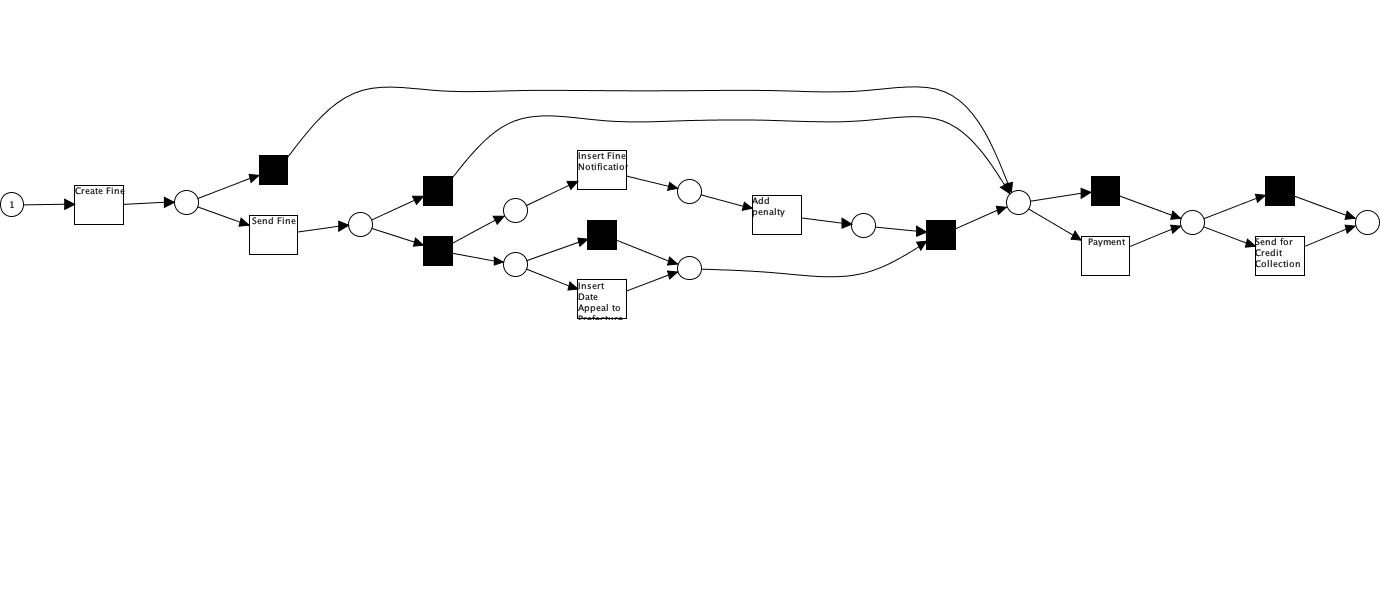
\includegraphics[width=\textwidth]{figures/im_no_appeals.png}
  \caption{Process model discovered from the log without any appeals using the inductive miner.}
  \label{fig:im_no_appeals}
\end{figure}
In respect to the given process the discovered model is simple and contains the most prominent process variants. The most important process paths can be seen at a glance. This subjective simplicity is supported by the computed simplicity value of 0.71. A number of possible process executions is not represented in the model. In general the model is very specific to the log and does not allow for much additional behaviour, it therefore subjectively does not generalize as well. Behaviours such as repeated activities (which is for example frequent for the \texttt{Payment} activity) are not modelled at all and can therefore not be expressed using the model. This tradeoff was chosen in order to obtain an easy-to-understand and simple model. This is important as we do not have access to domain experts, who might be able to better comprehend a model that allows for more behaviour.  However, the computed score for generalization of 0.91 is very good, this is probably caused by the many silent transitions that allow to skip many of the activities. 

For the sub-log containing only appeals cases, a different mining approach was applied at first. Instead of the Inductive Miner, the Interactive Data-Aware Heuristic Miner (IDHM) was used. This was done because the Inductive Miner resulted in a model that positioned many activities in a parallel construct, which reduced the amount of ordering information contained in the model. While the model discovered using the IDHM was better in that regard, it was neither safe nor sound. As we want to perform further analysis on the obtained model in future tasks, this is not ideal. Because of this problem of the IDHM approach, it was finally discarded. In order to obtain a sound model, the Inductive Miner was used again. The infrequent inductive miner approach of ProM was chosen, with a noise threshold of 0.1. By tweaking the noise parameter, it was possible to obtain a model that preserved more information about the ordering of activities. The final model can be seen in figure \ref{fig:im_appeals}.

\begin{figure}[H]
  \centering
  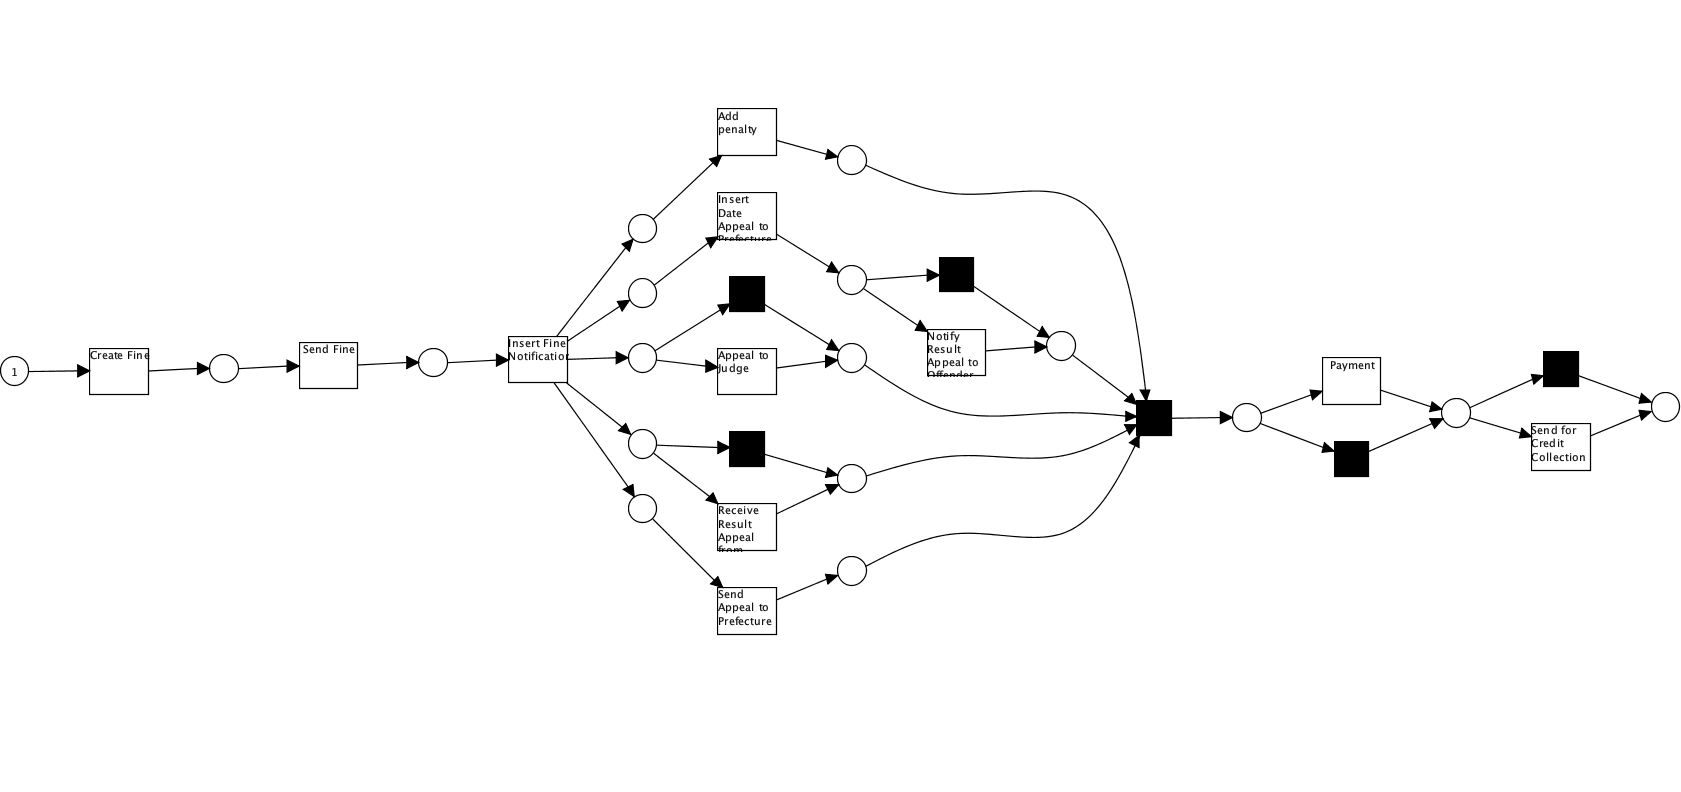
\includegraphics[width=\textwidth]{figures/im_appeals.png}
  \caption{Process model discovered from the log containing only appeals using the infrequent Inductive Miner.}
  \label{fig:im_appeals}
\end{figure}
Because there are more distinct activities, the discovered model is more complex than the model for cases without appeals that was discovered above. This is also represented in the computed simplicity score of 0.67 (compared to 0.71). However it can overall still be considered to be a simple model for the given process. Because of the large parallel construct in the middle of the model it is not extremely precise, however this also allows it to generalize well, as many different orderings of the activities are possible. The computed generalization score of 0.98 agrees with this subjective observation. Additionally the model is not able to cover more complex relationships between activities. It is for example possible to replay all cases regarding the \texttt{Payment} and \texttt{Send for Credit Collection} perfectly, because the activities are optional. The XOR relation that is present for these activities in the majority of cases is however not captured.

\paragraph{\textbf{b)}}
We applied the replay based and alignment based fitness measures to the two discovered models using pm4py. For the model containing no appeals we compute a replay based fitness of 0.99 and also an alignment based fitness of 0.99 (with 1 being the optimal value for both). We see that the model has an almost perfect fitness and is therefore able to describe most of the traces well. For the model of the other sub-log we obtain slightly lower fitness values of 0.97 (replay) and 0.97 (alignments), nevertheless the model has a very high fitness.

In order to judge the precision of the model we computed a score based on the escaping edges technique, which is also provided by pm4py. We obtain a value of 0.82 (with 1 being ideal) for the model that describes cases without appeals. For the model describing only cases with appeals, we obtain a value of 0.81. Based on these values we can conclude that both discovered models have a high precision.

\paragraph{\textbf{c)}}

We first consider the model for cases without appeals that can be seen in figure \ref{fig:im_no_appeals}. In the model all cases start with the \texttt{Create Fine} activity which is not optional. Directly following the first decision is made. It is now either possible that a large part of the process is skipped through a silent transition which leads to the end of the process, or that a reminder is sent to the offender (\texttt{Send Fine}). When skipping to the end, a construct consisting of the choice between \texttt{Payment} and \texttt{Send for Credit Collection} is reached. The model allows for one, both, or none of the activities to happen before reaching the final sink place. When a fine is sent to the offender, it is again possible to directly skip to the end construct when the offender pays quickly. Else the police department receives the notification of the reminder (\texttt{Insert Fine Notification}) and adds a penalty to the case (\texttt{Add Penalty}). Concurrently the offender makes an appeal to the prefecture (\texttt{Insert Date Appeal to Prefecture}). No appeal is initiated however, because the offender decides to make the payment, or the credit collection is made.

The model for the cases containing appeals can be found in figure \ref{fig:im_appeals}. The depicted process also starts with the \texttt{Create Fine} activity which is always followed by the \texttt{Send Fine} and \texttt{Insert Fine Notification} activities. Different activities now happen in parallel, without clear ordering. The penalty is added (\texttt{Add Penalty}), the appeal is send to the prefecture (\texttt{Send Appeal to Prefecture}, \texttt{Insert Date Appeal to Prefecture}). Sometimes the police department receives the result from the appeal and notifies the offender about it. Also optionally, in some cases the appeal to the judge is made (\texttt{Appeal to Judge}). After all of the described activities are concluded, the offender either pays the fine (\texttt{Payment}), or the fine is sent for collection. (\texttt{Send for Credit Collection}), according to the model it is also possible that both, or none of these activities happen (for example in cases where the appeal was successful).

\paragraph{\textbf{d)}}

For both of the models we do not expect a large amount of deviations, as the fitness of the models is very high. We start searching for deviations from the obtained process model in the log without appeals. The most frequent trace variant (2.6\% of traces) that cannot be represented by the model contains two \texttt{Payment} events at the end of the trace that directly follow each other. In these cases the offender has made two separate payments to pay the fine. Since this occurs in cases in which a penalty was added to the initial fine, we suspect that two separate payments are made for the fine and the penalty. This theory could be validated by comparing the \emph{amount} and \emph{paymentAmount} properties of the payment and fine events. We see that for all cases that follow the discussed variant, the \emph{paymentAmount} of the first payment was equal to the \emph{amount} of the fine and the second payment was equal to the \emph{amount} of the penalty. This means that in these cases, the offender most probably made the first payment before he was informed about the added penalty. 
There is a similar variant that also contains two \texttt{Payment} activities and makes up 2.3\% of the traces. In this variant first a payment is made, then a penalty is added and then a second payment occurs. Again the \emph{amount} and \emph{paymentAmount} of the events were investigated more closely to explain this deviation. We see that in most of these cases, the initial payment was only made for the fine, but was missing the expenses for the fine notification. Most probably the penalty was added because of the incomplete payment, but was then discarded as the offender corrected the first payment and payed the full amount. In addition the model is also not able to explain a payment activity that occurs before a penalty is added (if there is a penalty).The general problem of the model that we see in both of these cases however is, that it is not able to model multiple payment activities in one case. There are additional more infrequent variants that also experience multiple payment events.
In a different less frequent variant the payment is made directly after the fine is created, this can be explained by the model. However in these cases, a \texttt{Send Fine} event occurs after the payment. This cannot be expressed by the model. It was not possible to find a reason for this behaviour, since in all cases the fine was fully payed before the \texttt{Send Fine} event occurred. In many cases the event occurred many days after the payment, so there is no obvious reason for sending the fine.
Further deviations were not considered as they were extremely infrequent ($\leq 0.1\%$ of traces).

We now consider the model for the appeal cases. The first variant with a deviation comprises 3.0\% of the traces in the log. This variant consists of cases that are related to an appeal to a judge instead of an appeal to the prefecture and end with a payment. In these traces the prefecture related activities therefore do not happen. This is a problem for the \texttt{Insert Date Appeal to Prefecture} and \texttt{Send Appeal to Prefecture} activities which are not optional in the model, but do not occur in judge appeal cases. The same problem occurs in a similar variant (2.4\% of traces) that is identical to the discussed one, but ends with a credit collection.
A further deviation from the model is a variant that does not include the \texttt{Insert Fine Notification} and \texttt{Add Penalty} activities but rather directly inserts and sends the appeal to the prefecture (2.8\%) of traces. The absence of these activities is not able to be represented in the model.
These are all of deviations of the log from the model with a frequency $\geq 0.5\%$, additional there are several other variations of the judge appeal process. Overall we can conclude that the model is representing the process well and most of the deviations are related to the judge appeal process.

\paragraph{\textbf{e)}}

Based on the computed properties we can conclude that the two discovered models strike a reasonable balance between simplicity, fitness, generalization capability and precision and therefore can be reasonably used to describe the underlying processes. We observe that the model for the appeals process generally achieves worse scores for these metrics, which can be explained by the fact that it has fewer process instances and more possible activities. What is surprising in the appeals process model, is that there is a large number of parallel activities. This means that the order of the involved activities is ambiguous which is surprising in some cases. For example consider the \texttt{Insert Date Appeal to Prefecture}, \texttt{Send Appeal to Prefecture}, \texttt{Receive Result Appeal from Prefecture} \texttt{Notify Result Appeal to Offender} activities. They should reasonably occur in exactly this order, as it is not possible to receive the result before even sending the appeal. However this behaviour is possible according to the model. A closer inspection of the variants in the log reveals that this behaviour is not present in the actual log, where these activities happen in the correct order. The parallel construct can therefore be traced back to a shortcoming in the discovery algorithm and not an anomaly in the log.

The discovered model representing cases without appeals does not have such problems and in general scores higher on the computed metrics. While it suffers less from an arbitrary ordering of activities, it contains several silent transitions that make it possible to skip large parts of the process. We found that there are only little deviations from the model contained in the log. Most of these deviations are due to payment loops which are not represented in the model but to appear in reality. Further investigation revealed that in some cases the offender was confused about the amount that he owed due to the distinction between the fine amount and the expenses. A clearer wording in the fine documents that are send out to the offender might avoid these confusion, which could lead to a reduction in case duration in the future.

In general it appears that splitting the original event log into two sub-logs representing different kinds of process instances was a good choice that improved the quality of the obtained models greatly. While the two processes share the first activity and the choice construct between \texttt{Payment} and \texttt{Send for Credit Collection} in the end of the process, they differ greatly in the inner parts of the process. The split of the log made it possible to better comprehend these differing parts of the processes and made clear that there indeed is a significant difference between these two types of cases. A combined model would have been less simple and less precise as it would have mostly consisted of large parallel constructs and optional activities.

\section{Q3. Attribute Analysis and Compliance}

In this tasks we are analyzing the payment of Fines. For this purpose we are only interested in cases without appeal to overly complicate. We are assuming here that the activity \texttt{Send for Credit Collection} always ends in a complete payment of the Fine.

\paragraph{\textbf{a)}}

First of all we are investigating which fraction of fines gets payed properly and which fraction is over or under payed. We accomplish this by using a custom jupyter notebook. The total amount that has to be payed can be computed taking the maximum of the amount for the case and adding the sum of all expenses. By taking the maximal value of the column 'totalPaymentAmount' it is also possible to get the payments that the police department has received so far. Given these values it is possible to compute that approximately $80.3\%$ of traces result in a exact payment, $14.0\%$ of traces result in a no payment at all, $4.7\%$ of traces result in some but insufficient payment and $1.0\%$ of traces result in a over payment. All in all, this leads to a loss of $ \$ 1,438,950.6$ for the police department. Assuming that the police department eventually has to repay the over payments this loss rises to $ \$ 1,459,775.5 \$ $.

\section{Q4. Performance}

\paragraph{\textbf{a)}}

\begin{figure}[H]
  \centering
  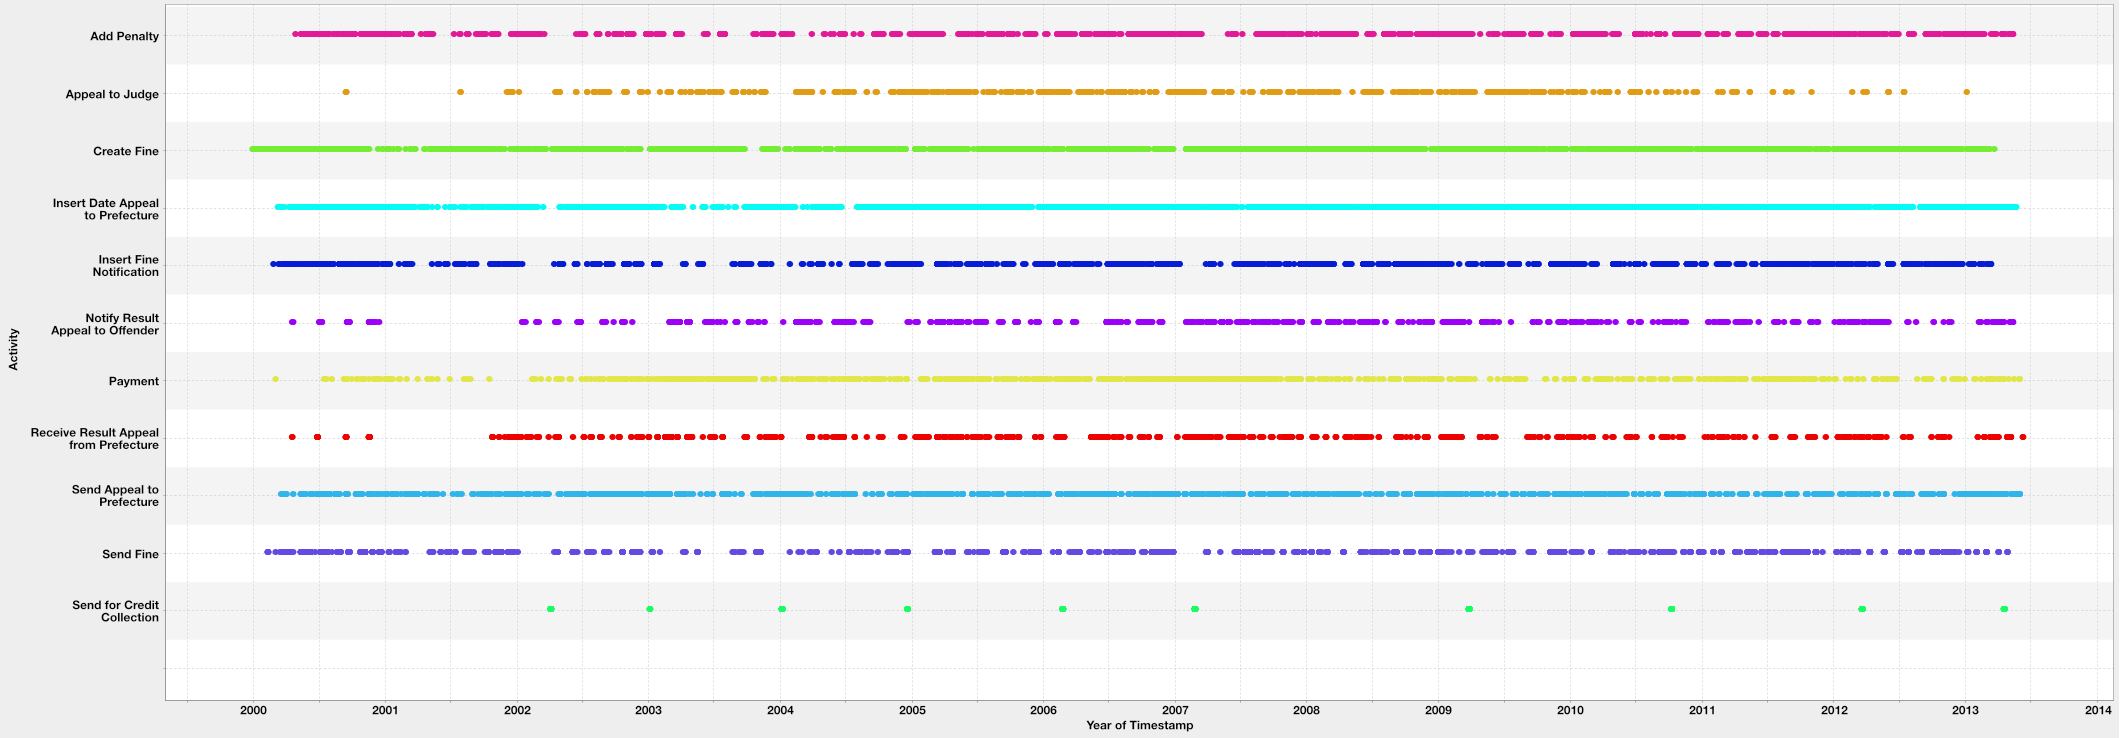
\includegraphics[width=\textwidth]{figures/dotted_timestamp_appeals.png}
  \caption{Event occurrences for cases with an appeal, grouped by activity type over time.}
  \label{fig:dotted_timestamp_appeals}
\end{figure}

\begin{figure}[H]
  \centering
  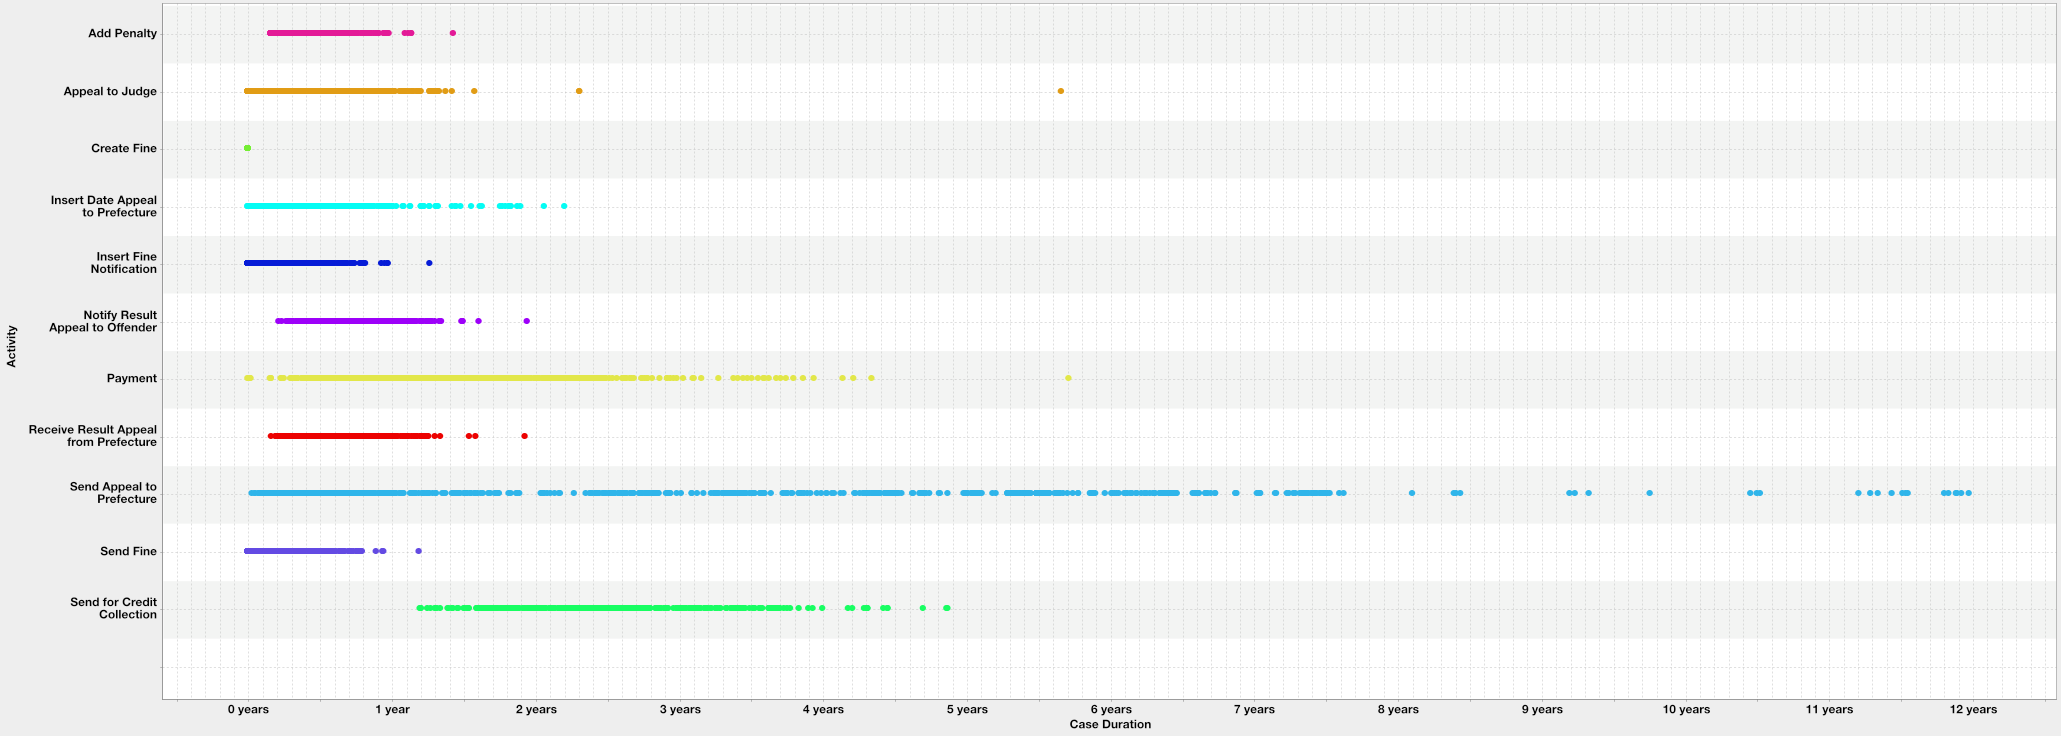
\includegraphics[width=\textwidth]{figures/dotted_duration_appeals.png}
  \caption{Event occurrences for cases with an appeal, grouped by activity type over the case duration at the time the event occurred.}
  \label{fig:dotted_duration_appeals}
\end{figure}

\paragraph{\textbf{b)}}

\paragraph{\textbf{b)}}

\section{Q5. Summary and Conclusion}

\section*{Appendix}

\begin{table}[H]
\centering
\begin{tabular}{|l|l|l|l|l|}
\hline \textbf{Activity} & \textbf{Complete} & \textbf{Only Appeals} & \textbf{Without Appeals} \\
\hline Add penalty & 79860 & 4357 & 75503\\
\hline Appeal to Judge & 555 & 555 &0\\
\hline Create Fine & 150370 & 4513 & 145857\\
\hline Insert Date Appeal to Prefecture & 4188 & 4146 & 42\\
\hline Insert Fine Notification & 79860 & 4357 & 75503\\
\hline Notify Result Appeal to Offender & 896 & 863 & 33\\
\hline Payment  & 77601 & 903 & 76698\\
\hline Receive Result Appeal from Prefecture & 999 & 964 & 35\\
\hline Send Appeal to Prefecture  & 4141 & 4141 & 0\\
\hline Send Fine  & 103987 & 4513 & 99474\\
\hline Send for Credit Collection & 59013 & 412 & 58601\\
\hline
\end{tabular}
\caption{Absolute Frequencies of Activities in the Event Logs}
\label{tab:1c_absolut}
\end{table}

\begin{table}[H]
\centering
\begin{tabular}{|l|l|l|l|l|}
\hline \textbf{Activity} & \textbf{Complete} & \textbf{Only Appeals} & \textbf{Without Appeals} \\
\hline Add penalty & 0.142234 & 0.146582 & 0.141991\\
\hline Appeal to Judge & 0.000988 & 0.018672 &0\\
\hline Create Fine & 0.267815 & 0.151830 & 0.274298\\
\hline Insert Date Appeal to Prefecture & 0.007459 & 0.139483 & 0.000079\\
\hline Insert Fine Notification & 0.142234 & 0.146582 & 0.141991\\
\hline Notify Result Appeal to Offender & 0.001596 & 0.029034 & 0.000062\\
\hline Payment  & 0.138210 & 0.030379 & 0.144238\\
\hline Receive Result Appeal from Prefecture & 0.001779 & 0.032432 & 0.000066\\
\hline Send Appeal to Prefecture  & 0.007375 & 0.139315 & 0\\
\hline Send Fine  & 0.185205 & 0.151830 & 0.187071\\
\hline Send for Credit Collection & 0.105104 & 0.013861 & 0.110205\\
\hline
\end{tabular}
\caption{Relative Frequencies of Activities in the Event Logs}
\label{tab:1c_relative}
\end{table}

\begin{table}[H]
\centering
\begin{tabular}{|l|l|l|l|l|}
\hline \textbf{Activity} & \textbf{Complete} & \textbf{Only Appeals} & \textbf{Without Appeals} \\
\hline Payment  & 0.446904 & 0.154443 & 0.455953\\
\hline Send for Credit Collection & 0.392346 & 0.087747 & 0.401770\\
\hline Send Fine  & 0.138026 & 0.001551 & 0.142249\\
\hline Send Appeal to Prefecture  & 0.020908 & 0.696654 & 0\\
\hline Appeal to Judge & 0.000891 & 0.029692 &0\\
\hline Notify Result Appeal to Offender & 0.000572 & 0.018170 & 0.000027\\
\hline Receive Result Appeal from Prefecture & 0.000352 & 0.011744 & 0\\
\hline
\end{tabular}
\caption{Fraction of Traces that end with the Corresponding Activity}
\label{tab:1c_end}
\end{table}

\end{document}

